\chapter{State of the Art}\label{chapter:StateOfArt}
CAPTCHA takes inspiration and is related to three main elements\cite{types_CAPTCHA}:
\begin{enumerate}
\descItem{Turing test}{it's used to determine how much a machine can think like a human. The test is made by three figures: a human examiner, an human and a machine. The examiner asks some questions to both other two figures and, after a fixed amount of time, evaluates if the two answers are different or not.\\
If they are similar w.r.t. the point of view of the examiner, the machine is an AI (Artificial Intelligence) similar to an human. The test is very important if the answers have many possibilities.}
\descItem{Human-Computer Interaction (HCI)}
{according to cognitive psychology studies, a human process data in a specific way and this test evaluates the interaction between humans and machines. The HCI model is divided into five levels:
\begin{itemize}
	\item{task level}
	\item{semantic level}
	\item{syntactic level}
	\item{interactive level}
	\item{a level of physical devices}
\end{itemize}   
Then the obtained information is processed by:
\begin{itemize}
	\item{reasoning}
	\item{problem solving}
	\item{skill acquisition}
	\item{error}
\end{itemize}   
}
\descItem{Human Interactive Proof (HIP)}
{it's used to make differentiation between machine and human users and computer user programs. The test require a type of interaction, that is simple to be done by human instead of bot. The main goals of this type of test are:
\begin{itemize}
	\item{To differentiate the humans from the computers}
	\item{To differentiate a category of the humans}
	\item{To differentiate a specific human from the category of humans}
\end{itemize}
HIP has the test program that is subjected to the human and the computer. As a result, only a specific group of humans can positively solve the test and then the test results can be validated by the computer.}
\end{enumerate}
In order to guarantee a good level of security, a CAPTCHA has to satisfy the following requirements:
\begin{itemize}
	\item{The solution to the CAPTCHA isn't conditional and shouldn't depend on the user's language and/or age.}
	\item{The solution of the CAPTCHA must be easy for the humans and hard for the bots. Hence, humans in no longer than 30 seconds with very high success rate}
	\item{The creation of the CAPTCHA must not disturb the user privacy (not linked to the user).}
\end{itemize}

%\vspace{4cm}
\section{Traditional CAPTCHAs}
The traditional CAPTCHAs are based on the knowledge and correct insertion of solution by the user. These CAPTCHA schemes are designed to exploit character recognition, image understanding and speech recognition to guarantee that the challenges will successfully block bots.\\
The main types of these CAPTCHAs are described in the following sections but the details about specific implementations can be found in the article of Walid Khalifa Abdullah Hasan\cite{survey_advanced_CAPTCHA}. With respect to user experience, the most enjoyable traditional CAPTCHAs are usually the game-based and image-based ones but the most frustrating CAPTCHA is the text-based one\cite{usability_CAPTCHA}. A summary of usability and security issues is shown in Table \ref{soa:traditional_table}.

\subsection{Audio-based CAPTCHAs}
This type of CAPTCHAs asks the user to type the words listened by an audio file (see Figure \ref{soa:audio_CAPTCHA}). It's developed for vision-impaired users. It usually has problems in usability related to the language dictionary, from which words are taken, and the similarity of the sound between several words. It has been proofed that this CAPTCHA is a hard task even for blind users, in fact  only 46\% of the challenges were solved by participants to an experiment\cite{usability_audio}.\\
One of the most popular CAPTCHAs is \textit{Audio reCAPTCHA}, developed at Carnegie Mellon University and then bought by Google. In this scheme, the user needs to recognize and write a set of 8 spoken characters from a noisy audio file with background voices. If the user makes a mistake, the test declares that he's a bot.\\
Audio-based CAPTCHAs are vulnerable to many Automatic Speech Recognition (ASR) programs\cite{improving_audio} but also Deep Learning techniques (e.g. DeepCRACk\cite{DeepCRACk}). A good overview about results, obtained by several classification methods, is described in the work of Jennifer Tam et al.\cite{break_audio}.
\begin{figure}[h]
     \centering
     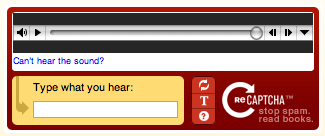
\includegraphics[width=.5\linewidth]{Images/StateOfArt/audio_CAPTCHA}
     \caption{\footnotesize{Example of audio-based CAPTCHA.}}\label{soa:audio_CAPTCHA}
\end{figure}

\subsection{Game-based CAPTCHAs}
This type of CAPTCHAs performs the verification of the user nature through a set of several kind of games (see Figure \ref{soa:game}). The strength of this CAPTCHAs is relative to the comprehension phase of the rules that only humans can perform.\\
This type of CAPTCHAs is called \textit{Dynamic Cognitive Game (DCG)} is usually developed using Flash and HTML5 with JavaScript. These technologies download the game code to the client and execute it locally.\\
The only difficult for the bot to attack the challenge is the encryption/obfuscation of the code. This strategy prevent the store of the code onto different internet domains. However for example, there exists a bot attack, called \textit{Stream Relay Attack}, that obtains good results bypassing these challenges \cite{game_CAPTCHA} (see Section \ref{soa:security_CAPTCHAs}).
\begin{figure}[h]
     \centering
     \begin{subfigure}[b]{0.48\textwidth}
         \centering
         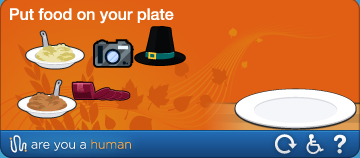
\includegraphics[width=.9\linewidth]{Images/StateOfArt/game_CAPTCHA}
     \end{subfigure}
     \hfill
     \begin{subfigure}[b]{0.48\textwidth}
         \centering
         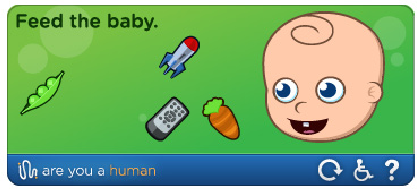
\includegraphics[width=.9\linewidth]{Images/StateOfArt/game_CAPTCHA2}
     \end{subfigure}
		
	 \begin{subfigure}[b]{0.55\textwidth}
         \centering
         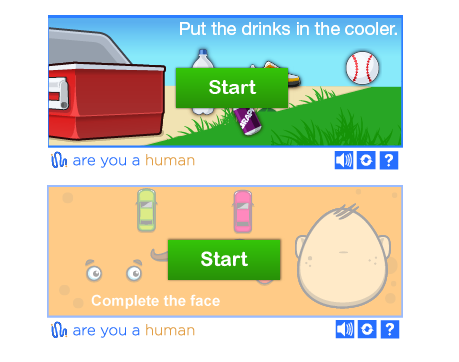
\includegraphics[width=\linewidth]{Images/StateOfArt/game_CAPTCHA3}
     \end{subfigure}
     \caption{\footnotesize{Examples of game-based CAPTCHAs.}}
     \label{soa:game}
\end{figure}

\subsection{Image-based CAPTCHAs}
Image-based CAPTCHAs require to understand a written text describing a task that needs an image evaluation to pass the test. This type of CAPTCHAs can be categorized into the following classes, looking to the task that the user needs to perform:
\begin{itemize}
\descItem{Click-based CAPTCHAs}
{this type of CAPTCHAs shows an image and a text that explains where the user needs to click (see Figure \ref{soa:click_CAPTCHA}).
\begin{figure}[h]
     \centering
     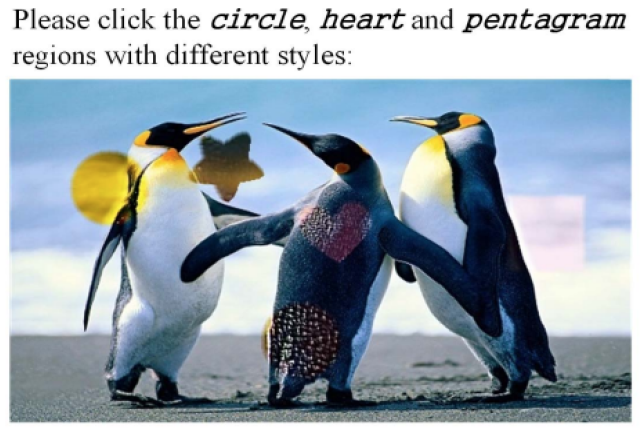
\includegraphics[width=.45\linewidth]{Images/StateOfArt/click_CAPTCHA}
     \caption{\footnotesize{Example of click-based CAPTCHA.}}\label{soa:click_CAPTCHA}
\end{figure}
}
\descItem{Sliding image-based CAPTCHAs}
{this type of CAPTCHAs asks the user to use the slider to solve an image-based challenge such as adjusting the orientation of an image, selecting the correct form of an image, or moving a fragment of an image to the correct location (see Figure \ref{soa:sliding_image}).
\begin{figure}[h]
     \centering
     \begin{subfigure}[b]{0.48\textwidth}
         \centering
         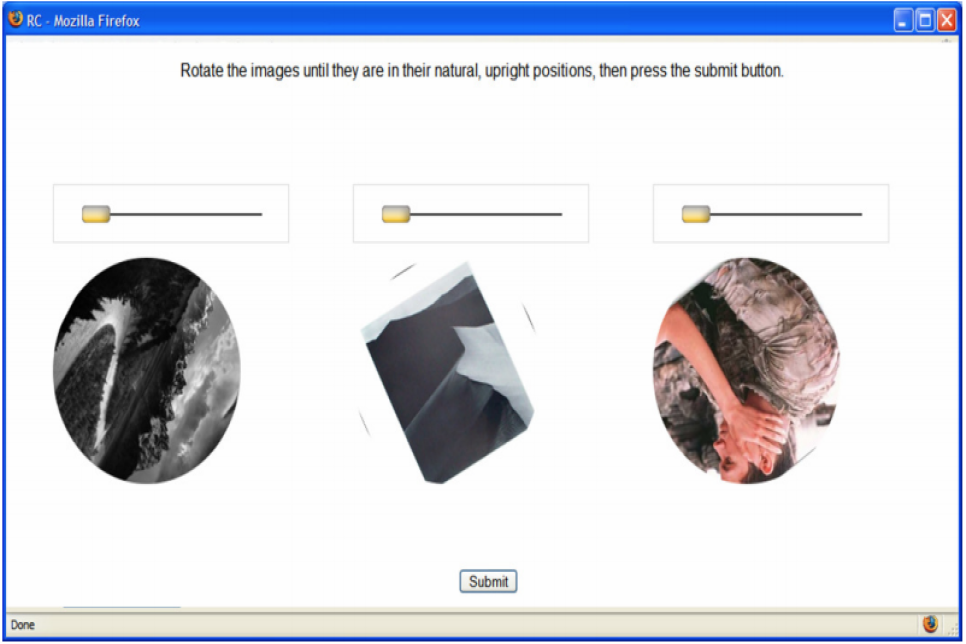
\includegraphics[width=.9\linewidth]{Images/StateOfArt/sliding_image_CAPTCHA}
	     \caption{\footnotesize{Orientation based.}}
     \end{subfigure}
     \hfill
     \begin{subfigure}[b]{0.48\textwidth}
         \centering
         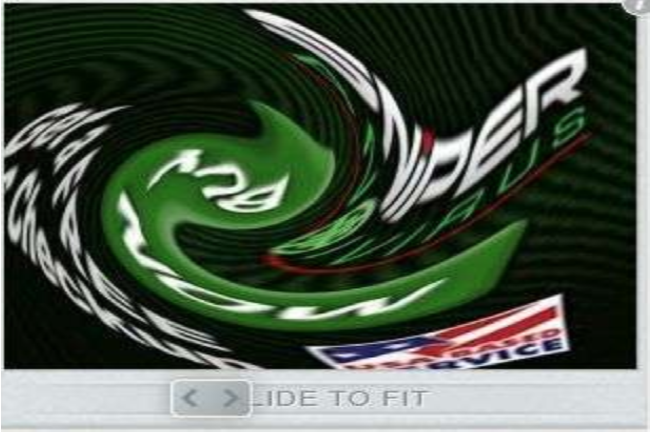
\includegraphics[width=.9\linewidth]{Images/StateOfArt/sliding_image_CAPTCHA2}
	     \caption{\footnotesize{Form based.}}
     \end{subfigure}
     \caption{\footnotesize{Examples of sliding image-based CAPTCHAs.}}
     \label{soa:sliding_image}
\end{figure}
}
\descItem{Drag \& Drop-based CAPTCHAs}
{this type of CAPTCHAs usually asks the user to complete a visual puzzle, created by dividing a given image in a set of pieces\cite{survey_CAPTCHA} (see Figure \ref{soa:puzzle}).\\
The task isn't easy for users because this type of CAPTCHAs takes more time to solve the puzzle but the security level is very high\cite{survey_CAPTCHA}. To improve the usability of the CAPTCHA, there exists a variant of the puzzle-based CAPTCHA in which needs to insert only some pieces of the puzzle instead of completing the whole puzzle (see Figure \ref{soa:puzzle2}).
\begin{figure}[h]
     \centering
     \begin{subfigure}[b]{0.48\textwidth}
         \centering
         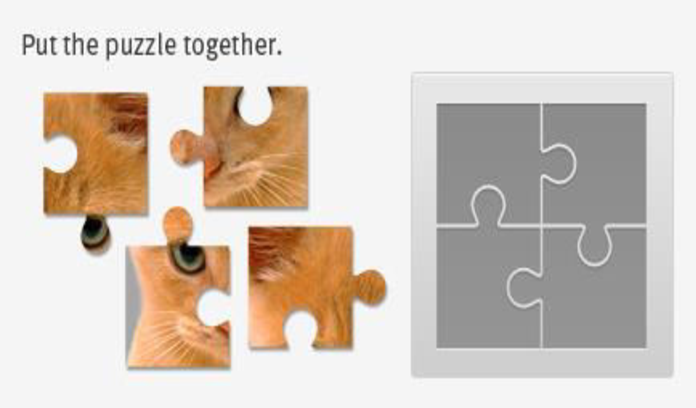
\includegraphics[width=.6\linewidth]{Images/StateOfArt/puzzle_CAPTCHA}
         \caption{\footnotesize{Completing the puzzle.}}
         \label{soa:puzzle}
     \end{subfigure}
     \hfill
     \begin{subfigure}[b]{0.48\textwidth}
         \centering
         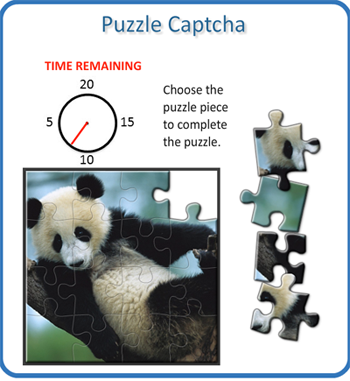
\includegraphics[width=.6\linewidth]{Images/StateOfArt/puzzle_CAPTCHA2}
         \caption{\footnotesize{Inserting only some pieces.}}
        \label{soa:puzzle2}
     \end{subfigure}
     \caption{\footnotesize{Examples of puzzle-based CAPTCHAs.}}
\end{figure}
}
\descItem{Selection-based CAPTCHAs}
{the user usually needs to select the images that contain a requested subject. The set of images, on which the user needs to identify the subject, can be implemented in different ways, for example:
\begin{itemize}
\item{An image is divided into a set of sub-squares and each of them is a candidate image\ref{soa:selection}}
\item{There are many images, each one with a unique different subject (see Figure \ref{soa:selection2})}
\end{itemize}
This type of CAPTCHAs is vulnerable to different Object Recognition techniques developed for Computer Vision purposes.\\
An extension of this type of CAPTCHAs, called \textit{FaceDCAPTCHA}, has been introduced\cite{FaceDCAPTCHA}. It incorporates elements of face detection. The human brain is very effective in the process of natural face segmentation even if there are complex backgrounds. This approach increases the security efficiency because the Computer Vision programs can easily detect if there is a face, e.g. Viola-Jones algorithm\cite{Viola_Jones}, but have many problems differentiating real and non-real photographs of faces.\\
Face, fingerprint and eye detections in images remain also a difficult challenge to be performed by computers. For this reason these results were used to develop a new variant of image-based CAPTCHA called \textit{MB CAPTCHA}\cite{MB_CAPTCHA}.
\begin{figure}[h]
     \centering
     \begin{subfigure}[b]{0.48\textwidth}
         \centering
         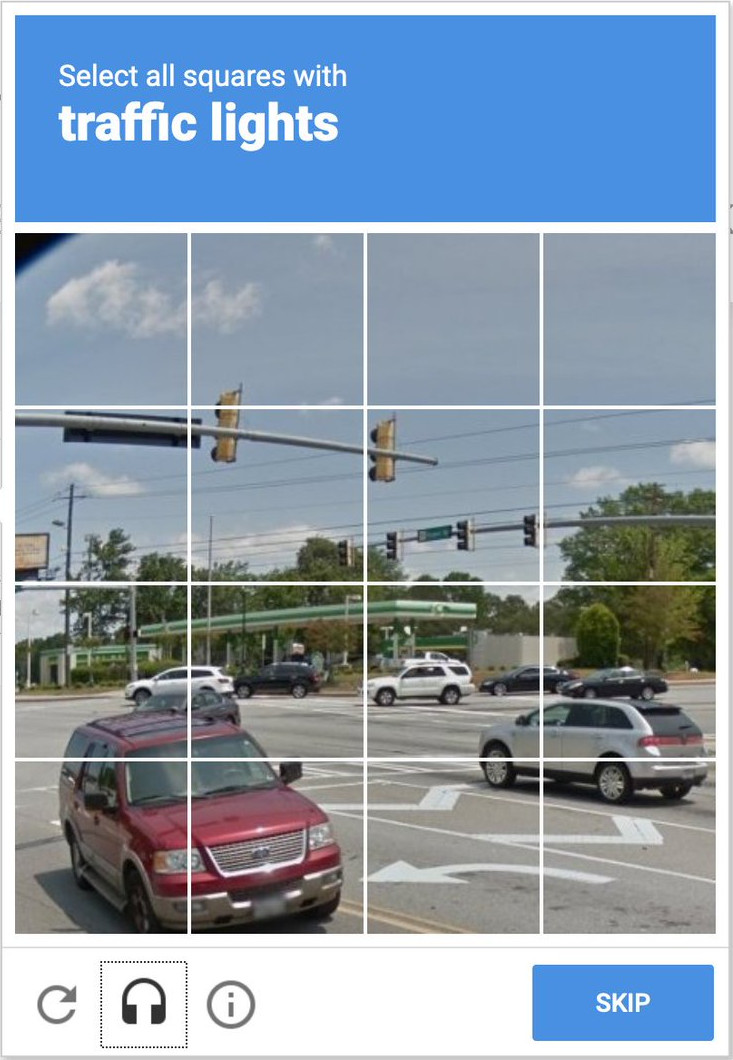
\includegraphics[width=.75\linewidth]{Images/StateOfArt/selection_CAPTCHA}
         \caption{\footnotesize{With an image divided in sub-squares.}}
         \label{soa:selection}
     \end{subfigure}
     \hfill
     \begin{subfigure}[b]{0.48\textwidth}
         \centering
         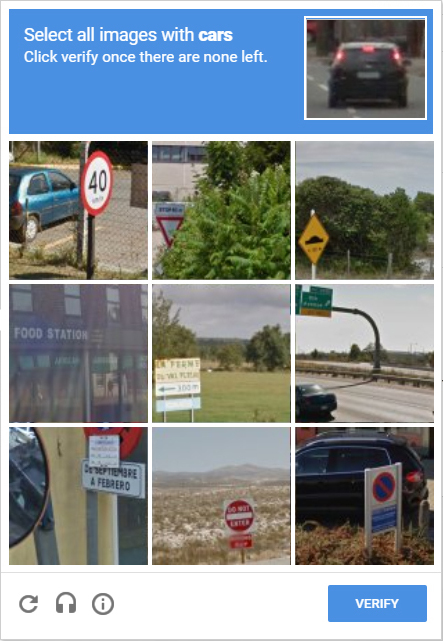
\includegraphics[width=.6\linewidth]{Images/StateOfArt/selection_CAPTCHA2}
         \caption{\footnotesize{With several images.}}
        \label{soa:selection2}
     \end{subfigure}
     \caption{\footnotesize{Examples of selection-based CAPTCHAs.}}
\end{figure}
}
\descItem{Interactive-based CAPTCHAs}
{the user needs to discover a secret position in an image using mouse movement or swiping gesture
\begin{figure}[h]
     \centering
     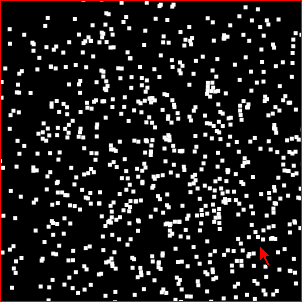
\includegraphics[width=.45\linewidth]{Images/StateOfArt/interactive_CAPTCHA}
     \caption{\footnotesize{Example of interactive-based CAPTCHA.}}\label{soa:interactive_CAPTCHA}
\end{figure}
}
\end{itemize}

\subsection{Math CAPTCHAs}
Looking to an operation specified in a frame, the user needs to insert the result in a text field. The operation is written in plain text or, to improve the security of this challenge, it's warped like text-based CAPTCHAs (Figure \ref{soa:arithmetic}). These classical math-CAPTCHAs, also known as \textit{arithmetic CAPTCHAs}, are vulnerable to OCR (Optical Character Recognition) techniques.\\
\begin{figure}[h]
     \centering
     \begin{subfigure}[b]{0.48\textwidth}
         \centering
         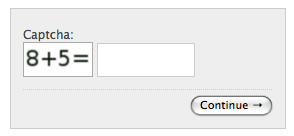
\includegraphics[width=.7\linewidth]{Images/StateOfArt/math_CAPTCHA}
         \caption{\footnotesize{With plain text.}}
     \end{subfigure}
     \hfill
     \begin{subfigure}[b]{0.48\textwidth}
         \centering
         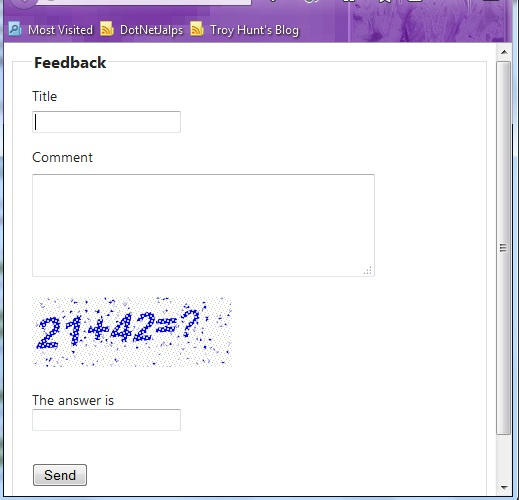
\includegraphics[width=.7\textwidth]{Images/StateOfArt/math_CAPTCHA2}
         \caption{\footnotesize{With wrapped text.}}
     \end{subfigure}
		\caption{\footnotesize{Example of arithmetic CAPTCHAs.}}
		\label{soa:arithmetic}
\end{figure}
An advanced version of this CAPTCHA is used in the Quantum Random Bit Generator Service (QRBGS) sign-up Web Page\cite{math_CAPTCHA} (see Figure \ref{soa:QRBGS}). This type of CAPTCHA asks user to solve an advanced math expression. It prevents the use of free or commercial OCRs because many mathematical symbols are not considered in their detection algorithm. However, it's vulnerable to side-channel attack \cite{math_CAPTCHA}.\\
Hence many math symbols are wrongly translated by bot programs and the challenge is very secure. The only problem is that this CAPTCHA is very complex for normal users and many of them could not solve the challenge correctly.
\begin{figure}[h]
     \centering
     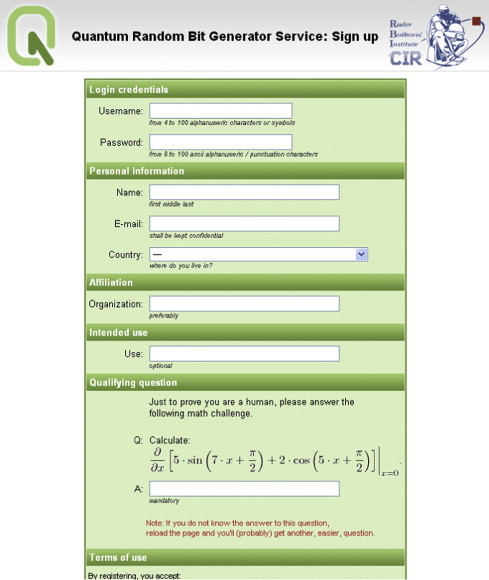
\includegraphics[width=.6\linewidth]{Images/StateOfArt/QRBGS}
     \caption{\footnotesize{Example of Quantum Random Bit Generator Service (QRBGS) sign-up Web Page \cite{math_CAPTCHA}.}}\label{soa:QRBGS}
\end{figure}

\subsection{Slider CAPTCHAs}
Slider CAPTCHAs only asks users to move the slider across the screen. Hence, image recognition is not part of the challenge to be classified as a human.\\
The most popular CAPTCHAs are the following:
\begin{itemize}
\descItem{CAPTCHA used by Taobao.com}{it asks the user to drag the slider from the start to the end of the sliding bar to verify his identity (see Figure \ref{soa:slider}).}
\descItem{CAPTCHA used by TheyMakeApps.com}{it asks the user to move the slider to the end of the line to submit a form\cite{sliding_CAPTCHA} (see Figure \ref{soa:slider2}).}
\end{itemize}
Different variations of this type of CAPTCHAs have been bypassed with a simple JavaScript code and puppeteer.
\begin{figure}[h]
     \centering
     \begin{subfigure}[b]{0.48\textwidth}
         \centering
         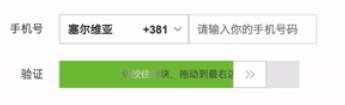
\includegraphics[width=.8\linewidth]{Images/StateOfArt/taobao_CAPTCHA}
                  \caption{\footnotesize{Example of TaoBao.com CAPTCHA.}}
         \label{soa:slider}
     \end{subfigure}
     \hfill
     \begin{subfigure}[b]{0.48\textwidth}
         \centering
         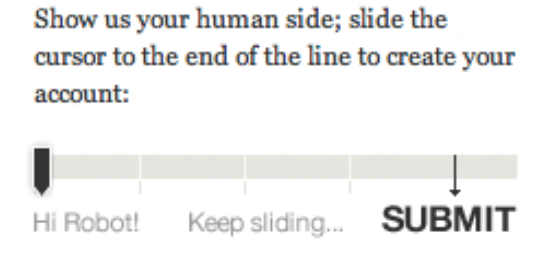
\includegraphics[width=.8\linewidth]{Images/StateOfArt/theyMakeApps_CAPTCHA}
         \caption{\footnotesize{Example of TheyMakeApps.com CAPTCHA.}}
        \label{soa:slider2}
     \end{subfigure}
     \caption{\footnotesize{Examples of slider CAPTCHAs.}}
\end{figure}

\subsection{Text-based CAPTCHAs}
In text-based CAPTCHA schemes a random series of wrapped characters and/or numbers is displayed on the screen inside an image(see Figure \ref{soa:text_CAPTCHA}). The user needs to understand which are the characters that composes the shown sequence and then type them inside a text-field. The text-based CAPTCHAs can be also classified in three main classes looking to the type of wrapped characters:
\begin{itemize}
\descItem{2D}{the digits are wrapped on a 2D plane, parallel to the screen plane}
\descItem{3D}{the digits are wrapped on a 3D plane oriented in the space and then a 2D image is taken from a specific point of view}
\end{itemize}
This type of CAPTCHAs is vulnerable to several type of attacks, related to Computer Vision techniques, that are:
\begin{itemize}
\item{OCR techniques\cite{OCR}}
\item{Segmentation techniques (e.g. DECAPTCHA\cite{DECAPTCHA})}
\item{Machine Learning and Deep Learning techniques}
\end{itemize}
In the design phase of a text-based CAPTCHA there are many issues, related to Computer Vision techniques, to be considered. For each of them, there is usually a solution in the design phase of the CAPTCHA that reduces the possibility that the challenge would be broken by a bot\cite{DECAPTCHA}.
\begin{figure}[h]
     \centering
     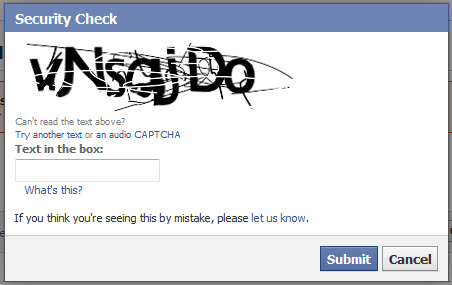
\includegraphics[width=.55\linewidth]{Images/StateOfArt/text_CAPTCHA}
     \caption{\footnotesize{Example of text-based CAPTCHA.}}\label{soa:text_CAPTCHA}
\end{figure}

\subsection{Video-based CAPTCHAs}
This type of CAPTCHA is not very common because of the weight of the file to be downloaded\cite{survey_advanced_CAPTCHA}. The traditional video-based CAPTCHA is composed by a video in which a sliding text is shown (see Figure \ref{soa:video}). The user needs to type this message in a text field to pass the challenge. Some implementations of this type of CAPTCHAs are vulnerable to machine learning attacks.\\
Another variant of this CAPTCHA is the \textit{Motion CAPTCHA}\cite{Motion_CAPTCHA}, developed by M. Shirali-shahreza and S. Shirali-shahreza, in which the user needs to watch a video. Then he needs to select which action was performed in the played file, choosing it from multiple answers (see Figure \ref{soa:video2}). The strength of these implementations of CAPTCHAs depends on the relationship between the multiple choices submitted to the user\cite{video_attack}.\\
A similar implementation of the previous variant, it's the one developed by Kluever et al. in which the user watches a video and needs to write three words that describe what he sees\cite{video_desc}. The same authors also performed a tag frequency-based attack to evaluate the security of their CAPTCHA schemes achieving a success rate of 13\%.
\begin{figure}[h]
     \centering
     \begin{subfigure}[b]{0.48\textwidth}
         \centering
         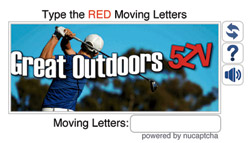
\includegraphics[width=\linewidth]{Images/StateOfArt/video_CAPTCHA}
         \caption{\footnotesize{Example of sliding text in video.}}
         \label{soa:video}
     \end{subfigure}
     \hfill
     \begin{subfigure}[b]{0.48\textwidth}
         \centering
         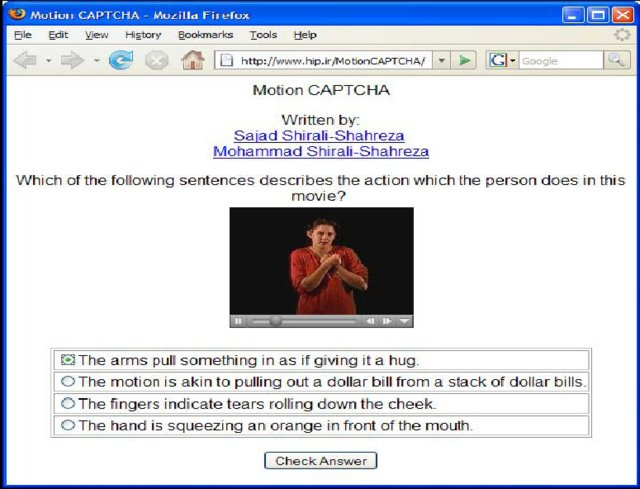
\includegraphics[width=\linewidth]{Images/StateOfArt/video_CAPTCHA2}
         \caption{\footnotesize{Example of Motion CAPTCHA\cite{Motion_CAPTCHA}.}}
        \label{soa:video2}
     \end{subfigure}
     \caption{\footnotesize{Examples of video-based CAPTCHAs.}}
\end{figure}

\section{Modern CAPTCHAs}
The type of CAPTCHAs and authentication mechanisms described in the following section are far from traditional CAPTCHAs and aren't based on cognitive knowledge of the human user but on other parameters, such as behavioural analysis and sensors readings. In the following sections there is a summary of the most known CAPTCHA schemes of this type.

\subsection{Biometrics-based CAPTCHAs}
The most known authentication mechanisms, that use biometric parameters of the user, are based on the following CAPTCHA schemes:
\begin{itemize}
\descItem{Bio-CAPTCHA voice-based Authentication}
{This authentication method was developed starting from good results reached in the authentication phase of cloud systems (Alexa for Amazon, Siri for Apple, Cortana for windows)\cite{voice_CAPTCHA}. This particular implementation uses a random voice-based password challenge. This password changes at every login of the user and this method uses CAPTCHA challenge to provide unpredictability and ambiguity to the authentication process. The experiments reveals that unauthorized access probability decreases, while it keeps high usability because it needs
only a mic.}
\descItem{rtCAPTCHA}{this type of authentication method is a Real-time CAPTCHA that asks users to perform some tasks like smile, blink or nod in front of the camera of the mobile phone. The recorded video is sent to the service provider that checks if in the file, there is the expected user performing the required action.\\
This implementation of CAPTCHA solves many problems of similar CAPTCHAs that are also based on liveness mechanisms and video capture. The attackers can extract patterns or features from existing or captured images and embed them into a new generated video in attack in the compromised device.\\
In the work of Erkam Uzun, Simon Pak Ho Chung, Irfan Essa and Wenke Lee\cite{rtCAPTCHA}, there is a detailed comparison between other similar authentication mechanisms and rtCAPTCHA, looking to all possible Computer Vision attacks.}
\end{itemize}

\subsection{Behavioural-based CAPTCHAs}
In 2014 Google announced that today’s Artificial Intelligence can solve even the most difficult variant of text-based CAPTCHAs at 99.8\% accuracy\cite{break_text}. For this reason, the company develops the following CAPTCHA schemes:
\begin{itemize}
\descItem{Google no CAPTCHA}
{Google developed in 2015 a new CAPTCHA system that is simpler than traditional CAPTCHAs in terms of user interaction\cite{google}. This CAPTCHA system is composed by two layers of protection:
\begin{enumerate}
\item{Checkbox \textit{"I'm not a robot"} to be clicked by user as in Figure \ref{soa:noCAPTCHA} (or image-based CAPTCHA on mobile devices)
\begin{figure}[h]
     \centering
     
\includegraphics[width=.4\linewidth]{Images/StateOfArt/noCAPTCHA}
     \caption{\footnotesize{Example of Google no CAPTCHA checkbox.}}\label{soa:noCAPTCHA}
\end{figure}
}
\item{Traditional text-based CAPTCHA with two warped words}
\end{enumerate}
The second layer is reached only if the user doesn't succeed in the first one. For the checkbox step, the application evaluates in background the user's behaviour (e.g. the mouse movement, where the users click, how long they linger over a checkbox). Then the program performs an \textit{advanced risk analysis}, by looking results of first step but also spam traffic and passed/failed CAPTCHAs. It understands in this way if the test is passed or not.\\
The tests done confirms that this phase was very inefficient and many times the first layer failed even if a human user was performing correctly the task. A problem of this type of CAPTCHA is that many attacks exploits the image-based CAPTCHA and text-based CAPTCHA using attacks based on known Computer Vision techniques or their variants (e.g. CAPTCHA breaker made by Suphannee Sivakorn, Jason Polakis and Angelos D. Keromytis\cite{break_google}).
}
\descItem{Google Invisible ReCAPTCHA}
{It's a top layer over the \textit{Google noCAPTCHA v2.0}, adding the option to bind directly to the form's submit element\cite{google}. It usually requires the use of cookies, used to track the user's behaviour. There exist two version of this CAPTCHA:
\begin{itemize}
\descItem{ReCAPTCHA v2.0}
{it was developed in 2017. It's not really invisible because Privacy \& Policy badge must be included on every page of app or website in which the CAPTCHA is used. Computer Vision and Artificial Intelligence algorithms can break the challenges by recognizing object in the pictures in the image-based CAPTCHA phase.}
\descItem{ReCAPTCHA v3.0}
{it was developed in 2018. With constantly analyzing human behavior, mouse movements, typing speed and other features incorporated into NO CAPTCHA technology, Google collected enough sample data to perfectly fine-tune their Google invisible reCAPTCHA v2.0 with this new version. This type of CAPTCHA uses Artificial Intelligence and Machine Learning probability scores, hostname, timestamp and anction validations.\\
Google removes image recognition and looking only the score, it evaluates if the user is a human or a bot. The main difference w.r.t. previous versions is that this CAPTCHA returns a probability score (\textit{risk score}) in the range $[0.0, 1.0]$: \textit{0.0} if the user is a bot, \textit{1.0} otherwise. The administrator of the website can decide what range of scores he wants to manage, declaring the the site is under attack and what actions need to be performed.\\
Some characteristics related to this version of \textit{Invisible ReCAPTCHA} are:
\begin{itemize}
\item{If a user accesses a Web page using incognito mode or private mode, he is classified with a very low score (\textit{high risk}).}
\item{If a human is wrongly classified as a bot, the user can login into its Google account to increase its score. If this doesn't change the classification, you cannot do anything else.}
\end{itemize}
}
\end{itemize}
}
\end{itemize}

\subsection{Sensor-based CAPTCHAs}
This type of devices have natively many sensors, like gyroscope and accelerometer, and the CAPTCHA schemes, described in the following sections, exploit their presence to improve security of the authentication.
\begin{itemize}
\descItem{Completely Automated Public Physical test to tell Computer and Humans Apart (CAPPCHA)}
{this is a way to enforce the PIN authentication phase by mobile phone\cite{CAPPCHA}. The user needs to tilt the device to a specified angle specified on the screen (see Figure \ref{soa:CAPPCHA}). The CAPPCHA security is based on the \textit{Secure Element} (\textit{SE}) present in the device. It prevents brute force, side channel and recording attacks. The usability results are good and then some of the comments made by users were considered in the implementation.
\begin{figure}[h]
     \centering
     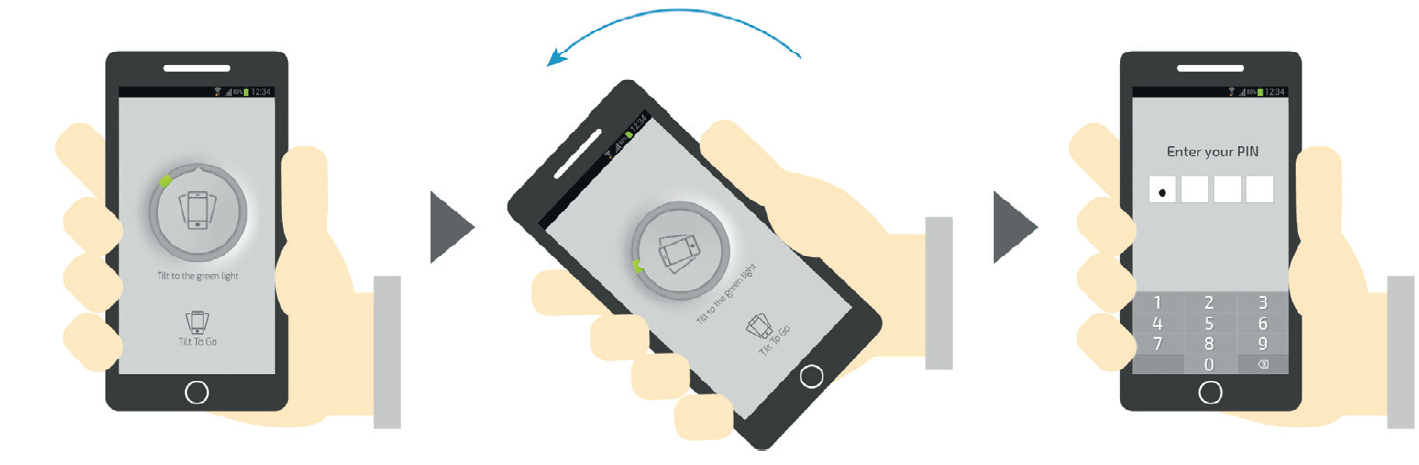
\includegraphics[width=.8\linewidth]{Images/StateOfArt/CAPPCHA}
     \caption{\footnotesize{CAPPCHA and PIN authentication\cite{CAPPCHA}.}}\label{soa:CAPPCHA}
\end{figure}
}
\descItem{Invisible CAPPCHA}
{It will be described in details in Chapter \ref{chapter:InvisibleCAPPCHA}.}
\end{itemize}

\section{CAPTCHA security}\label{soa:security_CAPTCHAs}
The process used for breaking CAPTCHAs is organized into the following phases\cite{CAPTCHA_attack_process}:
\begin{enumerate}
\descItem{Pre-processing phase}
{In this phase, several techniques are applied to remove background, separate foreground from the background, to delete noise and to remove some particular pattern (e.g. Canny Detection and Scale-Invariant Feature Transform (SIFT) application).
}
\descItem{Attack phase}
{the following techniques are usually applied:
\begin{itemize}
\descItem{\textit{Object Segmentation attacks}}
{Segmentation techniques (e.g. vertical histogram, colorfilling, snake segmentation and JSEG) are used to split the CAPTCHA image into segments to facilitate recognition}
\descItem{\textit{Object recognition attacks}}
{The most used techniques are pattern matching (e.g. shape context matching, correlation algorithm]), OCR recognition, SIFT and machine learning.}
\descItem{\textit{Random Guess Attacks}}
{The attacker's program tries to break the CAPTCHA scheme by guessing the correct answer. This attack is effective on CAPTCHAs with few number of different challenges.}
\descItem{\textit{Human Solver Relay Attacks}}
{The bot forwards the CAPTCHA challenge to a remote human worker that will solve it.}
\end{itemize}
}
\end{enumerate}
Many CAPTCHAs have yet the following known issues:
\begin{itemize}
\descItem{Session issue}
{Some types of CAPTCHAs have a big issue because they don't destroy the session, after the correct answer is inserted by the user\cite{text_audio}.\\
Hence, the hacker can crack following accesses using the same session id with the related solution of the challenge, after connecting to the web page of CAPTCHA. In this way the attacker can make hundreds of requests before the session expires and the previous operation must be computed again.}
\descItem{Resilience to both automated and human solver relay attacks}
{Many CAPTCHA schemes are designed to be robust against a possible AI attack but the new generation of CAPTCHA involves the use of remote bot or human solver. Traditional CAPTCHA schemes are vulnerable to this type of attacks.\\
Invisible reCAPTCHA and other academic proposals haven't been attacked yet, but works over thousands of different IP addresses and simulate the human behavior. Sensor-based CAPTCHAs are also vulnerable to solver relay attacks. An exception of this issue is the \textit{Invisible CAPPCHA}, that will be analysed in following sections and it's designed to block this type of attacks.
}
\descItem{Limited number of challenges}
{An issue of sensor-based CAPTCHA schemes is the limited number of challenges because the design of many usable gestures is very hard. This problem could be solved
relying on trusted hardware.}
\descItem{Trade-off between Friction-heavy and Frictionless CAPTCHAs}
{A trade-off between usability and security aspects is always considered analysing CAPTCHA schemes. This condition is highlighted in behavioural and sensor-based CAPTCHAs.}
\descItem{User's privacy}
{Sensor-based and behavioural CAPTCHAs usually send useful information to a remote server that analyses it to establish if the user was a human or a bot. If an hacker attacks the server side of this application, he can access to users' private data.\\
In some CAPTCHAs, the information are evaluated on the client side by a trusted hardware and the server receives only the results of the analysis. In this case, we need to be sure that trusted hardware is secure enough to guarantee privacy of user's information.
}
\descItem{Compatibility with different devices}
{Many CAPTCHA schemes, e.g. behavioural ones, use specific forms factors but a good challenge should be compatible with different factors.}
\end{itemize}

\begin{table}
\centering \footnotesize
\renewcommand*\arraystretch{1.3}
\begin{tabular}{ccll}
\toprule
\multicolumn{1}{c}{\textbf{Type}} & \multicolumn{1}{c}{\textbf{Scheme}} & \multicolumn{1}{c}{\textbf{Usability issues}} & \multicolumn{1}{c}{\textbf{Security}}\\
\midrule
%Audio row
\multirow{5}{*}{\textbf{\textit{Audio}}} & & {Issues of recognition:} & {It's vulnerable to:}\\
&&{\itemCell{Knowledge of English}}&{\itemCell{ASR programs.}}\\
&{\textit{Audio reCAPTCHA}}& {\hspace{1em}dictionary by the user.} &{\itemCell{Deep Learning and ML}}\\
&&{\itemCell{Some character sounds}}& {\hspace{1em}techniques.}\\
&& {\hspace{1em}very similar to others.} & \\
\midrule
\multirow{2}{*}{\textbf{\textit{Game}}} & {\textit{Dynamic Cognitive}} & {Comprehension of rules.} & {Vulnerable to Stream Relay}\\
& {\textit{Game (DCG)}} &&{Attack.}\\
\midrule
\multirow{5}{*}{\textbf{\textit{Image}}} & {\textit{Click-based}} & {Difficulty in identification} & {Vulnerable to:}\\
& {\textit{Drag \& Drop-based}} & {of images caused by:} & {\itemCell{Segmentation techniques}}\\
& {\textit{Sliding-based}} & {\itemCell{Blur of images.}} & {\itemCell{Deep Learning and ML}}\\
& {\textit{Selection-based}} & {\itemCell{Low vision condition.}} & {\hspace{1em}techniques}\\
& {\textit{Interactive-based}} &&{\itemCell{OCR techniques}}\\
\midrule
%Math row
\multirow{3}{*}{\textbf{\textit{Math}}} & {\textit{Arithmetic}} & {It requires basic or advanced} & {Vulnerable to:}\\
{} & {\textit{QRBGS}} & {math knowledge.} & {\itemCell{OCR techniques}}\\
&&&{\itemCell{Side-channel attacks}}\\
\midrule
\multirow{2}{*}{\textbf{\textit{Slider}}} & {Taobao.com} & {Simple and intuitive} & {Simple bypassed by Javascript}\\
& {TheyMakeApps.com} & {interaction.} & {code and pupeeteer.}\\
\midrule
\multirow{6}{*}{\textbf{\textit{Text}}} & & {Many problems have to} & {It can be identified by:}\\
&&{be solved by user:}&{\itemCell{OCR technique}}\\
&{\textit{2D}}&{\itemCell{Multiple fonts}}&{\itemCell{Segmentation techniques}}\\
&{\textit{3D}}&{\itemCell{Font size}}&{\itemCell{Deep Learning and ML}}\\
&&{\itemCell{Blurred Letters}}& {\hspace{1em}techniques}\\
&&{\itemCell{Wave Motion}}&\\
\midrule
{\textbf{\textit{Video}}} & {\textit{Motion CAPTCHA}} & {Heavy file to be downloaded} & {}\\
\bottomrule
\end{tabular}
\caption{\footnotesize{Survey of main types of traditional CAPTCHAs\cite{survey_CAPTCHA}.}}
\label{soa:traditional_table}
\end{table}

\begin{sidewaystable}
\centering \footnotesize
\renewcommand*\arraystretch{1.3}
\begin{tabular}{ccll}
\toprule
\multicolumn{1}{c}{\textbf{Type}} & \multicolumn{1}{c}{\textbf{Scheme}} & \multicolumn{1}{c}{\textbf{Usability issues}} & \multicolumn{1}{c}{\textbf{Security}}\\
\midrule
%Audio row
\multirow{3}{*}{\textbf{\textit{Audio}}} & {\textit{Audio reCAPTCHA}} & {Issues of recognition:} & {It's vulnerable to:}\\
&&{\itemCell{Knowledge of English dictionary by the user.}}&{\itemCell{ASR programs.}}\\
&&{\itemCell{Some character sounds very similar to others.}}&{\itemCell{Deep Learning and ML techniques.}}\\
\midrule
\multirow{2}{*}{\textbf{\textit{Game}}} & {\textit{Dynamic Cognitive}} & {Comprehension of rules.} & {Vulnerable to Stream Relay Attack}\\
& {\textit{Game (DCG)}} &&\\
\midrule
\multirow{5}{*}{\textbf{\textit{Image}}} & {\textit{Click-based}} & {Difficulty in identification of images caused by:} & {Vulnerable to:}\\
& {\textit{Drag \& Drop-based}} & {\itemCell{Blur of images.}} & {\itemCell{Segmentation techniques}}\\
& {\textit{Sliding-based}} & {\itemCell{Low vision condition.}} & {\itemCell{Deep Learning and ML techniques}}\\
& {\textit{Selection-based}} && {OCR techniques}\\
& {\textit{Interactive-based}} &&\\
\midrule
%Math row
\multirow{3}{*}{\textbf{\textit{Math}}} & {\textit{Arithmetic}} & {It requires basic or advanced} & {Vulnerable to:}\\
{} & {\textit{QRBGS}} & {math knowledge.} & {\itemCell{OCR techniques}}\\
&&&{\itemCell{Side-channel attacks}}\\
\midrule
\multirow{2}{*}{\textbf{\textit{Slider}}} & {Taobao.com} & {Simple and intuitive interaction} & {Simple bypassed by Javascript code}\\
& {TheyMakeApps.com} & {} & {and pupeeteer}\\
\midrule
\multirow{5}{*}{\textbf{\textit{Text}}} & {\textit{2D}} & {Many problems have to be solved by user:} & {It can be identified by:}\\
&{\textit{3D}}&{\itemCell{Multiple fonts}}&{\itemCell{OCR technique}}\\
&&{\itemCell{Font size}}&{\itemCell{Segmentation techniques}}\\
&&{\itemCell{Blurred Letters}}&{\itemCell{Deep Learning and ML techniques}}\\
&&{\itemCell{Wave Motion}}&\\
\midrule
{\textbf{\textit{Video}}} & {\textit{Motion CAPTCHA}} & {Heavy file to be downloaded} & {}\\
\bottomrule
\end{tabular}
\caption{\footnotesize{Survey of main types of traditional CAPTCHAs\cite{survey_CAPTCHA}.}}
\label{soa:traditional_table}
\end{sidewaystable}

\begin{comment}
\begin{sidewaystable}
\centering \footnotesize
\renewcommand*\arraystretch{1.3}
\begin{tabular}{ccll}
\toprule
\multicolumn{1}{c}{\textbf{Alternative Type}} & \multicolumn{1}{c}{\textbf{Name of implementation}} & \multicolumn{1}{c}{\textbf{Usability issues}} & \multicolumn{1}{c}{\textbf{Security}}\\
\midrule
\textit{} & {} & {}\\
\bottomrule
\end{tabular}
\caption{\footnotesize{Survey of main types of alternatives of CAPTCHAs\cite{survey_CAPTCHA}.}}
\label{soa:modern_table}
\end{sidewaystable}
\end{comment}